\documentclass{standalone}

\usepackage{tikz}
\usepackage{tkz-euclide}

\usepackage{times}

\usetikzlibrary {positioning}
\usetikzlibrary{arrows.meta}

\definecolor{hidden}{rgb}{0.6,0.6,0.6}
\definecolor{invalid}{rgb}{0.8,0.5,0.0}
\definecolor{valid}{rgb}{0.0,0.5,0.8}

\begin{document}
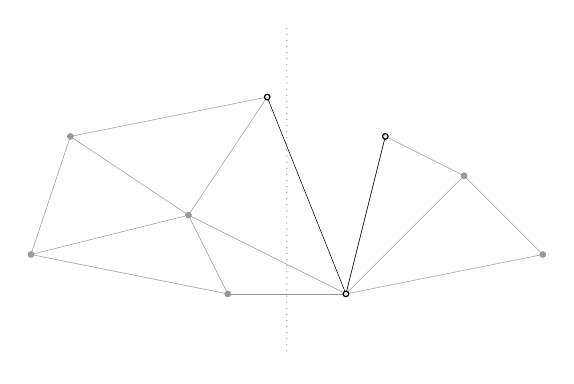
\begin{tikzpicture}

  \tkzDefPoint(-3.0,-0.5){min}
  \tkzDefPoint(4.5,3.0){max}

  % left half
  \tkzDefPoint(0.0,0.0){v0}
  \tkzDefPoint(0.5,2.5){v1}
  \tkzDefPoint(-2.0,2.0){v2}
  \tkzDefPoint(-2.5,0.5){v3}
  \tkzDefPoint(-0.5,1.0){v4}

  \tkzDrawSegments[hidden](v1,v2 v2,v3 v3,v0)
  \tkzDrawSegments[hidden](v0,v4 v1,v4 v2,v4 v3,v4)

  % right half
  \tkzDefPoint(1.5,0.0){v5}
  \tkzDefPoint(4.0,0.5){v6}
  \tkzDefPoint(3.0,1.5){v7}
  \tkzDefPoint(2.0,2.0){v8}

  \tkzDrawSegments[hidden](v5,v6 v6,v7 v7,v8 v8,v5 v5,v7)

  \tkzDefLine[mediator](v0,v5)\tkzGetPoints{p}{q}
  \tkzDrawLine[dotted,add=0.8 and -0.2](p,q)

  \tkzDrawSegments(v5,v1)

  \tkzDrawSegment(v5,v8)

  \tkzDrawSegments[hidden](v0,v5 v5,v4)

  \tkzDrawPoints[hidden](v0,v1,v2,v3,v4,v5,v6,v7,v8)
  \tkzDrawPoints(v1,v5)
  \tkzDrawPoints(v8)
  %\tkzLabelPoints(v0,v1,v2,v3,v4,v5,v6,v7,v8)

\end{tikzpicture}
\end{document}
